Machine learning is a field which is evolving quickly and therefore a lot of papers have been published in the last few years. However, since focus of this master thesis is on generating adversarial examples, related work can be separated into two topics, depending if a DNN is treated as a white-box or a black-box. 

In terms of white-box attacks, in \cite{fgsm-original}, the \textit{Fast Gradient Sign Method} is presented. It computes an adversarial image for a non-targeted attack based on the direction of the gradient of a DNN. It is presented in the Section \ref{sec:FGSM}.

In \cite{DBLP:journals/corr/PapernotMJFCS15}, the \textit{Jacobian-based Saliency Map Attack} JSMA algorithm for generating adversarial examples is presented. It is based on identifying regions in an image which have higher importance for a DNN during the classification. It is presented in the Section \ref{sec:JSMA}.

In \cite{DBLP:journals/corr/CarliniW16a}, the CW attack is presented which is based on formulating the attack as an optimization problem and using a state-of-the-art optimizer to solve it.  It is presented in the Section \ref{sec:CW}.

All three attacks, FGSM, JSMA and CW are used in the experiments in this thesis.

On the black-box side of the attacks, there is \textit{transfer-based} approach 
\cite{DBLP:journals/corr/PapernotMGJCS16}. It uses a subsitute DNN which is trained on a similar dataset as the targeted DNN. This approach is described in the Section \ref{sec:transfer-based}.

In \cite{ensemble-attack}, the authors show that adversarial samples for targeted misclassification don't transfer as well as in a pure misclassification attack. Authors suggest \textit{ensemble} approach which is described in the Section \ref{sec:ensemble-approach}.

In \cite{brendel2018decisionbased}, authors implement a completely different attack and call it \textit{Boundary Attack}. The attack starts with an image of a targeted class and then, step by step, it changes it to an image of some other class while staying adversarial, i.e. classified as a target class by a DNN under the attack. The attack is described in the Section \ref{sec:boundary-attack}.

I direct the interested reader to this survey for a detailed description \cite{survey} of the different attack strategies and defenses.

\section{Fast Gradient Sign Method (FGSM)}
\label{sec:FGSM}
Let $\pmb \theta$ be the parameters of a model, $\pmb x$ the input to the model, $y$ the target associated with $\pmb x$, and $J (\pmb \theta, \pmb x, y)$ be the cost fucntion used to train the neural network. Then an adversarial perturbation is computed as 
\[ 
\pmb \rho = \epsilon * sign (\nabla_{\pmb x} J(\pmb \theta, \pmb x, y)).
\]

An adversarial example can be crafted then by adding the adversarial perturbation to the original input

\[\pmb x = \pmb x + \pmb \rho .\]
 
 
The FGSM attack perturbs an image to increase the loss of the classifier on the resulting image. The target label in the original paper \cite{fgsm-original} was always a label with the least probability for an unmodified image. The authors evaluate their method on the ImageNet dataset \cite{datasetImageNet}, a dataset used for a large-image recognition task with 1000 classes, and achieve good results for misclassification. Targeted misclassification was not evaluated. Similar results are achieved on the MNIST dataset 	\cite{datasetMNIST}, a dataset used for a digit-recognition task (0-9), and on the CIFAR-10 dataset \cite{datasetCIFAR10}, a dataset used for a small-image recognition task, also with 10 classes as in MNIST. From Figure \ref{fig:gibbon}, a reader can get the intuition for the attack. For more details, please consult the original paper.

\begin{figure}[h]
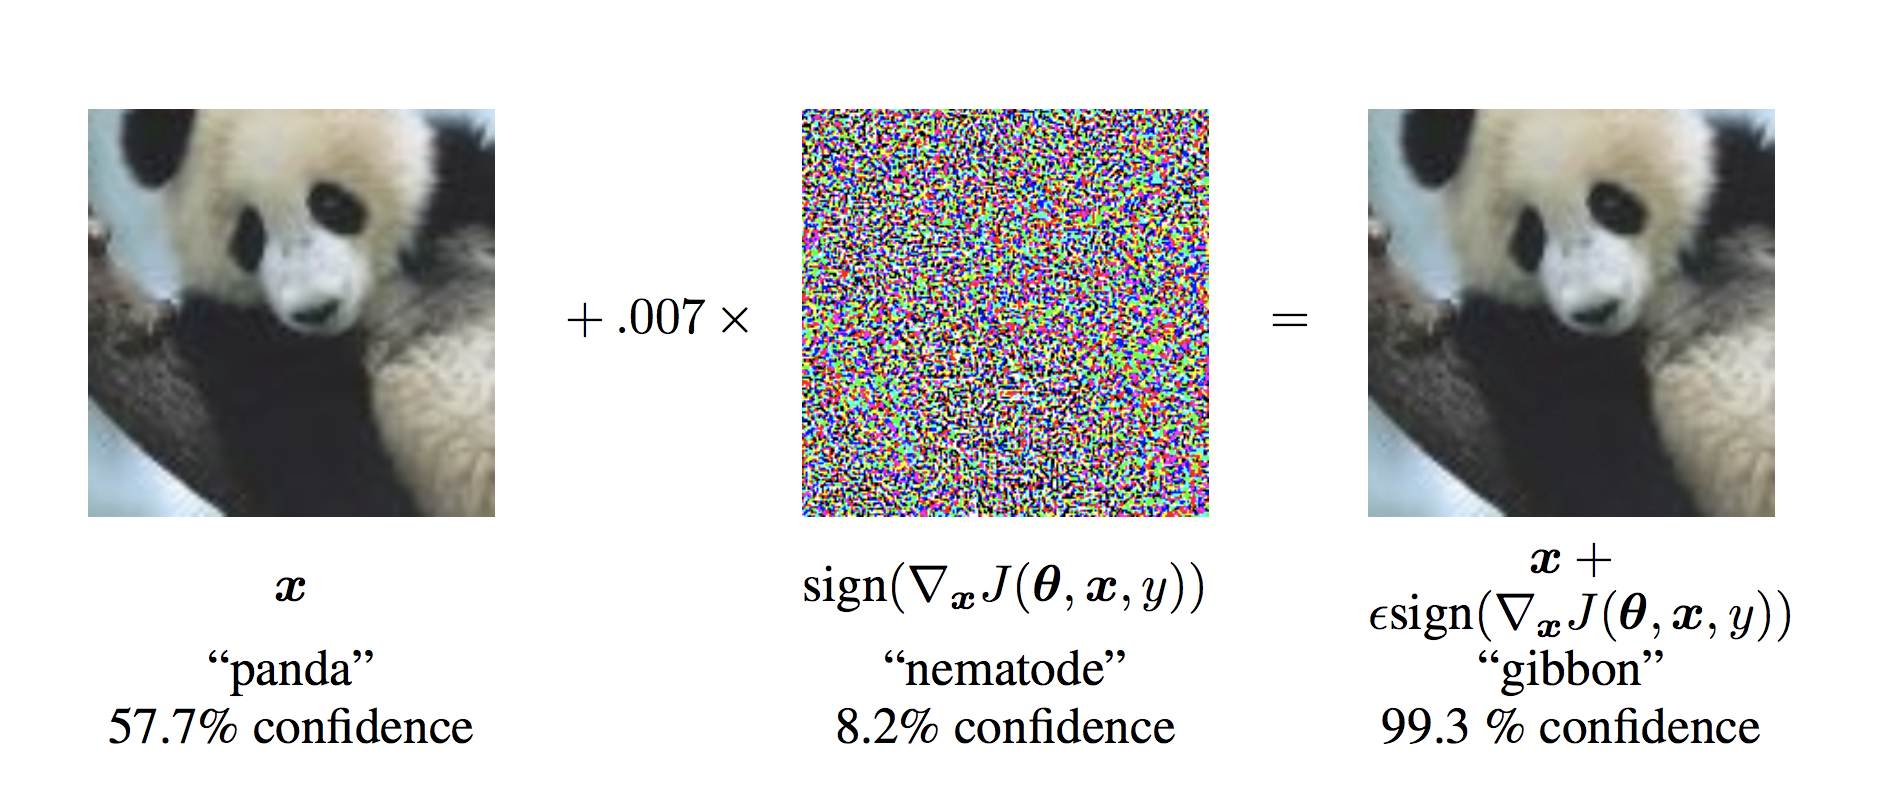
\includegraphics[width=13cm]{gibbon}
\caption{Image taken from the \cite{fgsm-original}}
\label{fig:gibbon}
\end{figure}




\section{Jacobian-based Saliency Map Attack (JSMA)}
\label{sec:JSMA}
This attack is based on a greedy algorithm that picks pixels to modify one at a time, increasing the the likelihood of the targeted class in each iteration.  \textit{Adversarial Saliency Maps} - maps that measure an impact of a pixel on an image being classified as a target class - are created. If a value in this map is large, it means that changing that pixel will increase the likelihood of the image being classified as a target class. 

The idea is, given the saliency map for a target class, the algorithm picks the pixel with the highest impact and modifies it. In the next iteration, the second most important pixel is changed and so on. This continues until either the attack succeeds to trick the classifier or too many pixels get changed and the attack becomes detectable. In the actual implementation of the algorithm, instead of picking one pixel, a pair of pixels is picked.

Formally, let $t$ be the target class, $\pmb x$ be the input to the classifier and $\pmb F$ be the output of the softmax layer. Then the adversarial saliency map in terms of pair pixels $p, q$ is defined as:

\[
\alpha_{pq} = \sum_{i \in \{p,q\}} \frac{\partial \pmb F(\pmb x)_t}{\partial \pmb x_i},
\]

\[
\beta_{pq} = ( \sum_{i \in \{p,q\}} \sum_{j \neq t} \frac{\partial \pmb F (\pmb x)_j }{\partial \pmb x _i}) - \alpha_{pq}
\]

so that $\alpha_{pq}$ represents the impact of changing the both pixels $p$ and $q$ on the input being classified as $t$, and $\beta_{pq}$ represents how
much changing $p$ and $q$ will change all the other outputs of the softmax layer.

Now the algorithm picks $p$ and $q$ such that the target class gets more likely ($\alpha_{pq} > 0$), but other classes get less likely ($\beta_{pq} < 0$) and that combination is as strong as possible, i.e. that $ - \alpha_{pq} * \beta_{pq}$ is as large as possible. This can be formalized as:

\begin{align*}
(p^*, q^*) 
				&= arg max_{p, q} (- \alpha_{pq} * \beta_{pq}) \\
                  & \textnormal{ s.t. } \alpha_{pq} > 0 \textnormal{ and } \beta_{pq} < 0
\end{align*}


Starting with an original input, two by two pixels are picked and perturbed by a constant offset $\epsilon$. The authors \cite{DBLP:journals/corr/PapernotMJFCS15} show that JSMA attack can effectively produce MNIST samples that are correctly classified by human subjects, but misclassified into a specific target class by a DNN with a high success rate. 

 
\section{Carlini \& Wagner (CW)}
\label{sec:CW}
% L norm introduction

To quantify similarity between two images, different distance metrics can be used. Quantification of similarity can be used when comparing how much an adversarial image is different from the original input. There are three widely-used distance metrics in the literature for generating adversarial examples , all of which are $L_p$ distances. The $L_p$ distance is written $||x - x'||_p$, where the $p$-norm is can be defined as

\begin{equation}
  ||v||_p=\left\{
  \begin{array}{@{}ll@{}}
       |\{i | v_i \neq 0 \}|, & \text{if } p = 0 \\
    ( \sum_{i = 1}^{n} |v_i|^p)^{1/p}, & \text{if } p \in [1, \infty) \\
    max\{|v_1|, |v_2|, ..., |v_n|\} & \text{if } p = \infty
  \end{array}\right.
\end{equation} 

In other words, $L_0$ measures how many pixels are changed, $L_2$ measures standard euclidean distance and $L_\infty$ measures the maximum change to any of the coordinates. It is open for discussion which metric performs the best job in measuring the human perceptual of similarity, but neither of the $L_p$ metrics is optimal for that.

% end of L norm introduction

The authors \cite{DBLP:journals/corr/CarliniW16a} introduce three new attacks for the $L_0$, $L_2$, and $L_{ \infty }$ distance metrics. It is worth mentioning that their $L_0$ attack is the first published attack which can cause targeted misclassification on the ImageNet dataset. All three of them are based on optimization techniques.

In this thesis, $L_2$ is used in the attack and hence I explain it now.

Let $t$ be the target class, $\pmb Z$ be the output of the targeted DNN before the softmax layer with $\pmb Z_i$ as an output for the class $i$, $\kappa$ a parameter that controls the confidence with which the misclassification occurs, $c$ a constant value, and $\pmb x$ be the original input.
Given $\pmb x$ and the target class $t$, search for $\omega$ that solves

\[
argmin_{\omega} ||\frac{1}{2}*(tanh(\omega) + 1) - \pmb x||_2^2 + c * f(\frac{1}{2}(tanh(\omega) + 1))
\]
with $f$ defined as 
\[
f(\pmb x') = max(max\{\pmb Z(\pmb x ')_i : i \neq t\} - \pmb Z(x)_t, - \kappa).
\]

The unrestricted perturbation $\pmb \delta^*$ is then defined as 
\[
	\pmb \delta^*_i = \frac{1}{2} * (tanh ( \omega_i) + 1) - \pmb x_i
\]
and after converting it to the restricted perturbation $\pmb \delta$ (details in the original paper \cite{DBLP:journals/corr/CarliniW16a}), an adversarial example $\pmb x^*$ is produced as 
\[
\pmb x^* = \pmb x +\pmb  \delta.
\]

According to the authors, this attack is often much more effective (and never worse) than all the others presented in the literature. Attacks are evaluated on the three datasets: ImageNet, MNIST and CIFAR-10. They also report that the JSMA attack, an attack introduced in Section \ref{sec:JSMA}, is always failing on the ImageNet dataset due to memory complexity of the algorithm, i.e. dimensions of images in ImageNet dataset are too big for JSMA attack. This implies that the JSMA attack would not work in my thesis as well if an image of a person is too big. Reported results for the CW attack are showing 100\% success against all three datasets.










\section{Transfer based approach}
\label{sec:transfer-based}
This technique is used to attack the DNN in the black-box settings. The idea is to create a \textit{substitute} DNN which should be similar to the targeted DNN. A precise definition of the similarity is omitted here because it's not well defined, but the substitute DNN should solve the same task as the targeted DNN.

Adversarial images are crafted then for a substitute DNN using a white-box approach, for instance the FGSM attack introduced in Section \ref{sec:FGSM}. Created adversarial images are used then as adversarial images for the black-box DNN as well. The main idea is that similar classifiers will have similar boundaries for a specific class and therefore the same adversarial example should be adversarial for both networks. 

The dataset on which the substitute neural network is trained should be similar to the dataset on which the targeted neural network is trained. Ideally, that would be the same dataset, but the assumption is that an attacker doesn't have access to that data. 

The attacker therefore generates a Synthetic Dataset. He or she starts generating the dataset by querying the targeted DNN with several examples and obtaining labels for them. Afterwards, he or she expands the dataset using the Jacobian-based Dataset Augmentation and trains the substitute neural network. For more details how to generate the synthetic dataset, please consult the original paper  \cite{DBLP:journals/corr/PapernotMGJCS16}.

The Authors present good results for misclassification attacks against the MNIST dataset and the GTSRD dataset \cite{datasetGTSRD}. Targeted misclassification is not presented in the paper.


\section{Ensemble approach} 
\label{sec:ensemble-approach}
This approach is also based on transferability of an adversarial image, but instead of generating an adversarial image for one neural network, generates it for several of them. The underlying assumption is that if an adversarial example works as expected among several models, it will work as expected for the one more as well. Both approaches will be implemented - when a substitute network is only a single neural network, and when there is several of them. I want to see if it's enough to use only one neural network as a substitute to achieve good results in semi-targeted misclassification.



\section{Boundary attack}
\label{sec:boundary-attack}
This approach is also used in black-box settings and it is completely different than attacks introduced in Sections \ref{sec:transfer-based} and \ref{sec:ensemble-approach}. Boundary attack has nothing to do with neither a substitute DNN nor transferability of the adversarial examples. 

The attack starts with an image of a targeted class and then, step by step, it changes it to an image of some other class while staying adversarial, i.e. classified as a target class by a DNN under the attack. In every iteration of the attack, the image is changed a little bit towards a class which will be in the image in the end, at least according to a human observer. 

After every change, the targeted DNN is queried to check if the image is still adversarial, i.e. classified as a target label. If not, the change is reverted. In this way, the attacker doesn't need any substitute neural network. 

However, this attack comes at cost of number of queries to the targeted DNN. For the targeted attack, the authors needed around $10^4$ queries to get an adversarial example. The real world systems could notice such intensive querying of their APIs and detect the attack. On top of that, the attacker needs both: an image of the targeted class and an image of the class for a human observer. That could be an obstacle when the number of classes is high because it can happen that it is not easy to find an image of a particular class.

The authors \cite{brendel2018decisionbased} compare boundary attack with white-box CW attack, introduced in Section \ref{sec:CW}, on MNIST and CIFAR-10 dataset and produce only a bit worse results, although this attack is treating a targeted DNN as a black-box.  For more information about this approach, please consult the original paper \cite{brendel2018decisionbased}.

